\documentclass{../exhibit}

\title{Hop Along, Matey!}

%% Font
\usepackage{imfellEnglish}
\usepackage[T1]{fontenc}
\raggedright

\usepackage{background}

\backgroundsetup{
scale=1,
color=black,
opacity=0.4,
angle=0,
contents={%
  \includegraphics[height=\paperheight]{mapBackground.jpg}%%https://upload.wikimedia.org/wikipedia/commons/8/81/Nautical_chart_of_the_West_Indies_1797.jpg
  }%
}




%% For the context
%% https://tex.stackexchange.com/questions/86150/torn-page-effect/86151#86151
\usepackage{tikz}
\usetikzlibrary{decorations.pathmorphing}
\definecolor{paper}{RGB}{239,227,157}





\renewcommand{\maketitle}{ %
  \begin{center}
    \scalebox{8}{\thetitle}
  \end{center}
  
\begin{tabular*}{\textwidth}{c @{\extracolsep{\fill}} c}  
\resizebox{4in}{!}{\begin{minipage}[b]{3in}\huge\directions\end{minipage}} &
  \resizebox{4in}{!}{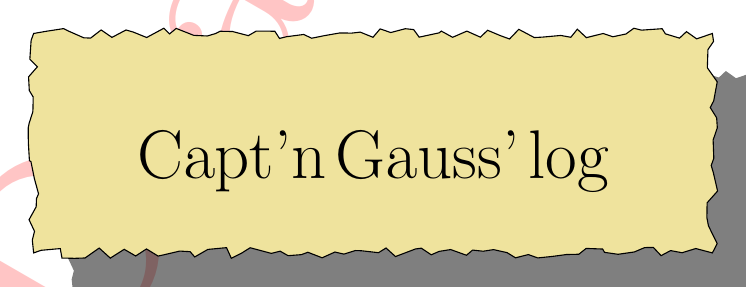
\begin{tikzpicture}[pencildraw/.style={ %
    decorate,
    decoration={random steps,segment length=4pt,amplitude=2pt}
    } %
]
\node[
preaction={fill=black,opacity=.5,transform canvas={xshift=.5cm,yshift=-.5cm}},
pencildraw,draw,fill=paper,text width=3in,inner sep=.5cm] 
{\begin{center}\Huge Capt'n Gauss' log \end{center}\vspace{.7cm} {\huge\context}};
\end{tikzpicture}}

\end{tabular*}

\vfill

\includegraphics[width=3in]{logoPirate.png}\hfill \includegraphics[width=2in]{bammLogo.png}


}


\begin{document}

\begin{context}
Are ye tired of counting yer treasure one by one? Well, have no fear, for I have a secret technique for ye to speed up yer counting. It's called \textbf{skip counting!}
\end{context}

\begin{directions}
There will be tape on the floor marking out numbers.

Try hopping over every other number to count 1, 3, 5, 7, \ldots

Or try hopping onto every third number to count 1, 4, 7, 10, \ldots

\end{directions}

\begin{example}
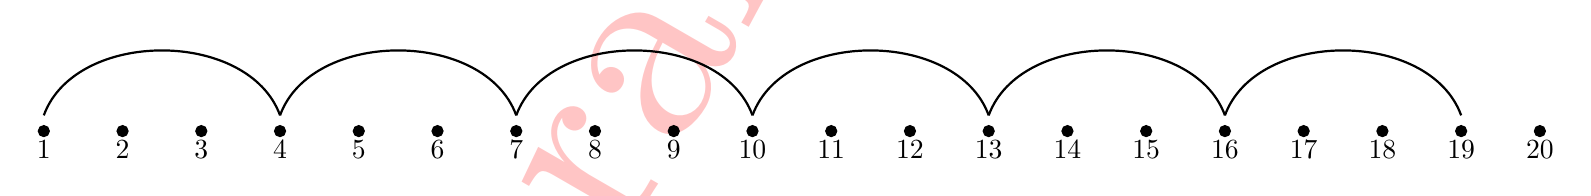
\begin{tikzpicture}

\foreach \x in {1,2,3,...,20} {
    \filldraw (\x,0) circle (2pt);
    \node[below] at (\x,0) {\x};
}
\foreach \x in {1,4,7,...,16} {
  \draw [thick] (\x,0.2) edge [in=110,out=70] ({\x+3},0.2);
}

\end{tikzpicture}
\end{example}

\begin{mathConnections}
  https://bartsnapp.github.io/Math-Outreach-Exhibits/skipCounting/
\end{mathConnections}
\end{document}
